\usepackage{amsthm}
\usepackage{amsfonts}
\usepackage{amsmath}
\usepackage{amssymb,bbm}
\usepackage{dsfont}
\usepackage{bm}
\usepackage{graphicx}
\usepackage{algorithm}
\usepackage{algorithmic}

\usepackage{color}

\newcommand{\R}{\mathbb{R}}
\newcommand{\one}{\mathds{1}}
\newcommand{\mat}[1]{\mathbf{#1}}
%\renewcommand{\vec}[1]{\mathbf{#1}}
\renewcommand{\vec}[1]{\bm{#1}}

%%Title:
\title{An Inexact Penalty Method for Fast Unbalanced \protect\\ Optimal Transport Optimization}

%%Contact address:
\address{ Xun Su, Waseda University, 3-4-1 Okubo, Shinjuku-ku, Tokyo 169-8555, Japan}

%%Name of authors:
\author{%
Xun Su\first
\and
Hiroyuki Kasai\second
}

%%Affiliations:
\affiliate{
\first{} WASEDA University, Department of Communications and Computer Engineering, Graduate \protect\\School of Fundamental Science and Engineering\\
\second{}WASEDA University, Department of Communications and Computer Engineering, School of \protect\\ Fundamental Science and Engineering
}

%%
%\Vol{28} %% <-- 25
%\session{0A0-00}%% <-- ID

\begin{abstract}
With the increasing application of Optimal Transport (OT) in machine learning, the unbalanced optimal transport (UOT) problem, as a variant of optimal transport, has gained attention for its improved generality. There is an urgent need for fast algorithms that can efficiently handle large penalty parameters. In this paper, we propose to use the Inexact penalty to make the Majorize-Minimization algorithm converge quickly even in UOT with large penalties. By using a dynamic scheme, we can successfully compute better and sparser solutions for the large penalty parameter and approach the computational speed of the well-known Sinkhorn algorithm, which sacrifices accuracy by adding an entropy item.
\end{abstract}

%\setcounter{page}{1}
\def\Style{``jsaiac.sty''}
\def\BibTeX{{\rm B\kern-.05em{\sc i\kern-.025em b}\kern-.08em%
T\kern-.1667em\lower.7ex\hbox{E}\kern-.125emX}}
\def\JBibTeX{\leavevmode\lower .6ex\hbox{J}\kern-0.15em\BibTeX}
\def\LaTeXe{\LaTeX\kern.15em2$_{\textstyle\varepsilon}$}

\begin{document}
\maketitle

\section{Introduction}
\label{sec:int}

Optimal transport (OT) has gained popularity in the fields of machine learning and statistical learning due to its ability to measure the distance between two probability measures. New methods that combine OT have outperformed traditional methods in areas such as domain adaptation \cite{Courty_PAMI_2017} and generative models \cite{arjovsky2017wasserstein}. The rise in popularity of OT is largely due to the introduction of Sinkhorn's algorithm \cite{Cuturi_NIPS_2013} for the entropy-regularized Kantorovich formulation problem, which has reduced the computational burden associated with large-scale problems.

Despite its success, the standard OT problem has a limitation in that it only handles {\it balanced} samples. To accommodate a wider range of applications with {\it unbalanced} samples, the unbalanced optimal transport (UOT) \cite{Caffarelli_AM_2010,chizat2017scaling} has been proposed. UOT replaces the equality constraints with a KL divergence as a penalty function, and it is solvable by adding an entropic regularization term and using Sinkhorn's algorithm. Although it is fast, scalable, and differentiable, it suffers from instability, larger errors in solution compared to other regularizers.

Recently, \cite{Chapel_NeurIPS_2021} proposed a Majorization-Maximization Algorithm to solve the UOT problem without adding an entropy part by considering the mutual connection between the UOT problem and the non-negative matrix factorization problem. The algorithm is computable in GPU form, similar to Sinkhorn's algorithm, but it is still slower, especially for large penalization terms.

In this paper, we propose to combine the inexact penalty method, which was first introduced by \cite{pmlr-v115-xie20b} in the OT community and has been adapted in Augmented Lagrangian methods for many years, with the MM algorithm, to speed up the optimization process. Our method is simple and effective, and can greatly improve the computational speed of the MM algorithm with larger penalization terms.

\section{Algorithm}
\subsection{Preliminaries}
We use $\| \cdot \|_2$ to represent the Euclidean norm. $\mathbb{R}^n$ denotes $n$-dimensional Euclidean space, and $\mathbb{R}^n_+$ denotes the set of vectors in which all elements are non-negative. $\mathbb{R}^{n \times m}_+$ stands for the set of $n \times m$ matrices in which all elements are non-negative. We present vectors as bold lower-case letters $\vec{a},\vec{b},\vec{c},\dots$ and matrices as bold-face upper-case letters $\mat{A},\mat{B},\mat{C},\dots$. The $i$-th element of $\vec{a}$ and the element at the $(i,j)$ position of $\mat{A}$ are stated respectively as $a_i$ and ${A}_{i,j}$. In addition, $\one_n \in \mathbb{R}^n$ is the $n$-dimensional vector in which all elements are one.
%For $\vec{x}$ and $\vec{y}$ of the same size, $\langle \vec{x},\vec{y} \rangle = \vec{x}^T\vec{y}$ is the Euclidean dot-product between vectors.
For two matrices of the same size $\mat{A}$ and $\mat{B}$, $\langle \mat{A},\mat{B}\rangle={\rm tr}(\mat{A}^T\mat{B})$ is the Frobenius dot-product. We use $\|\vec{a}\|_2$, $\|\vec{a}\|_1$, and $\|\vec a\|_{\infty}$ to represent the $\ell_2$-norm, $\ell_1$-norm, and $\ell_{\infty}$ norm of $\vec{a}$, respectively.

\subsection{Backgrounds}
The balanced OT problem is defined as
\begin{eqnarray}
\label{Eq:Standard_OT}
\operatorname{OT}(\vec{a},\vec{b}) &:=& \min_{ \mat{T} \in \R_{+}^{n \times m}} \langle \mat{C}, \mat{T} \rangle \\
\text{subject\ to}&& \mat{T} \one_n= \vec{a}, \mat{T}^{T}\one_m = \vec{b}, \notag
\end{eqnarray}

By adding the KL divergence to penalize the difference, The UOT problem is defined as:
\begin{eqnarray}
\label{eq:uot}
\operatorname{UOT}(\vec{a},\vec{b}) := \min_{\mat{T} \in \R_{+}^{n \times m}} \langle \mat{C}, \mat{T} \rangle \\
+ \tau KL(\mat{T} \one_n,\vec{a}) + \tau KL(\mat{T}^{T} \one_n,\vec{b}).
\end{eqnarray}

\cite{Chapel_NeurIPS_2021} considered the UOT probelm as a composite optimization problem. They propose the MM algorithm to solve the UOT problem:

\begin{eqnarray}
\label{eq:update}
\mat{T}^{(k+1)}&=\operatorname{diag}\left(\frac{\vec a}{\mat{T}^{(k)} \one_m}\right)^{\frac{1}{2}}\left(\mat{T}^{(k)} \odot \exp \left(-\frac{\mat C}{2 \lambda}\right)\right)\\
& \operatorname{diag}\left(\frac{\vec{b}}{\mat{T}^{(k) \top} \one_n}\right)^{\frac{1}{2}},
\end{eqnarray}
It is noteworthy that the updating formula \ref{eq:update} bears striking similarities with the widely popular Sinkhorn Algorithm, relying solely on matrix multiplication. This allows a GPU acceleration for faster computation.
\subsection{Proposed Method}
However, we observed that the MM algorithm suffers from performance degradation for larger $\tau$ values, as illustrated in {\bf Fig.~\ref{Fig:ex2}}. Similarly, the Augmented Lagrangian Method (ALM) also uses an additional quadratic penalization term to expedite convergence but is plagued by an ill-conditioned Hessian matrix \cite{doi:10.1137/1.9781611973365}.
To overcome these limitations, we introduce a novel Inexact Penalized MM algorithm (MM-IP) that incorporates a dynamic penalization term, gradually increasing its influence throughout the optimization process. This approach has been previously employed in ALM research, and we demonstrate its effectiveness in our proposed algorithm.
In {\bf Algorithm.~\ref{Alg1}}, we set a small constant $q$ and gradually increase the value of $\tilde{\tau}$ as the optimization error reduces. This inexact optimization process enables our algorithm to obtain a sparser initialization, allowing it to avoid the ill-conditioned Hessian matrix issue encountered in the early stages of optimization.
\begin{algorithm}[t]
\caption{Inexact Penalty Method UOT}
\begin{algorithmic}[t]
\label{Alg1}
\renewcommand{\algorithmicrequire}{\textbf{Input:}}
\renewcommand{\algorithmicensure}{\textbf{Output:}}
\REQUIRE $\mat{T}^0, \mat C, \tilde{\tau}, \tau, q$
\ENSURE $\mat T^{K}$
\STATE $\mat G = \operatorname{exp}(-\frac{C}{2\tilde{\tau}})$
\FOR {$k = 1 \text{ to } K$}

\STATE $u = (\frac{a}{\mat T \one_n})^{\frac{1}{2}}, v=(\frac{b}{\mat{T}^{T} \one_m})^{\frac{1}{2}}$
\STATE $\mat{T}^{k} = \mat T^{k} \odot ( u^{T} \mat G v)$
\STATE $err = \|\mat T^{k-1} - \mat T^{k}\|_2$
\IF {$err \leq \frac{q}{\tilde{\tau}} \text{ and } \tilde{\tau} \leq \tau$}
\STATE $\tilde{\tau} = \min(\tau, 2 *\tilde{\tau})$
\ENDIF
\ENDFOR
\end{algorithmic}
\end{algorithm}

Since $\tilde{\tau}$ only doubles during the MM-IP algorithm for $O(log(\tau))$ times, the computation burden for recomputing matrix $\mat K$ is ignorable compared with the MM algorithm.

\section{Experiments}
We use Random Generated Gaussian distribution to test our method. In {\bf Fig.~\ref{Fig:ex1}}, we present the results of our experiment, where we generate five pairs of 100-dimensional random Gaussian distributions. We apply linear programming to obtain the analytical optimal solution $\mat T^{*}$ for the mass-equal pairs. For our experiments, we set $\tau = 1000$, and we use Sinkhorn's algorithm (UOT) with a regularizer value of $\epsilon = 1e-3$ to compute the solution. We also set the initial value of $\tilde{\tau} = 0.1$ and $q = 10^{-4}$ for our Inexact Penalized MM algorithm (MM-IP). We further apply Nesterov acceleration to our algorithm to obtain AMM-IP.

2 experiments demonstrate that the MM algorithm struggles to optimize the transport cost for the large penalization parameter, resulting in a significantly higher error than other methods. This can be observed in {\bf Fig.~\ref{Fig:ex2}}, where the large value of $\tau$ forces the optimization algorithm to converge to a dense solution, which is worse than both Sinkhorn algorithm and our proposed methods.
\begin{figure}[t]
\centering
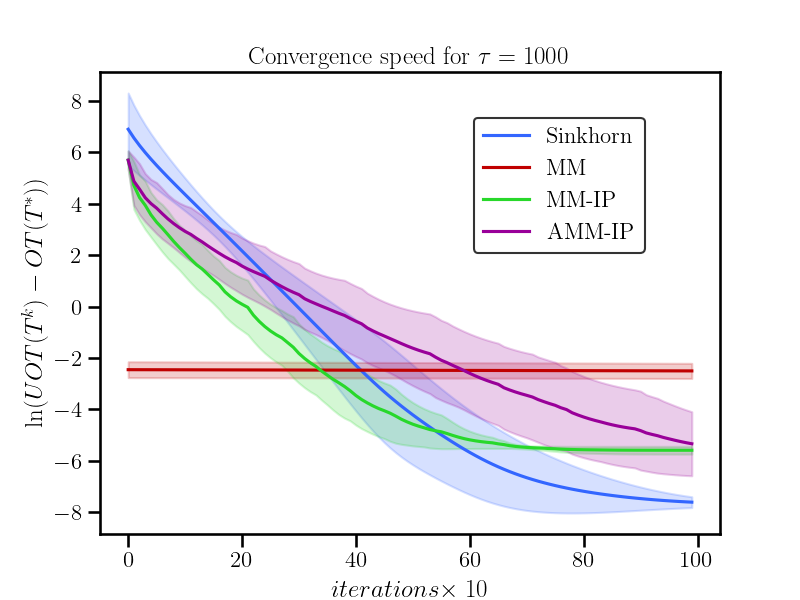
\includegraphics[width = 0.9\linewidth]{pic/ex1}
\caption{Comparing of the convergence speed for different projection methods.}
\label{Fig:ex1}
\end{figure}
\begin{figure}[t]
\centering
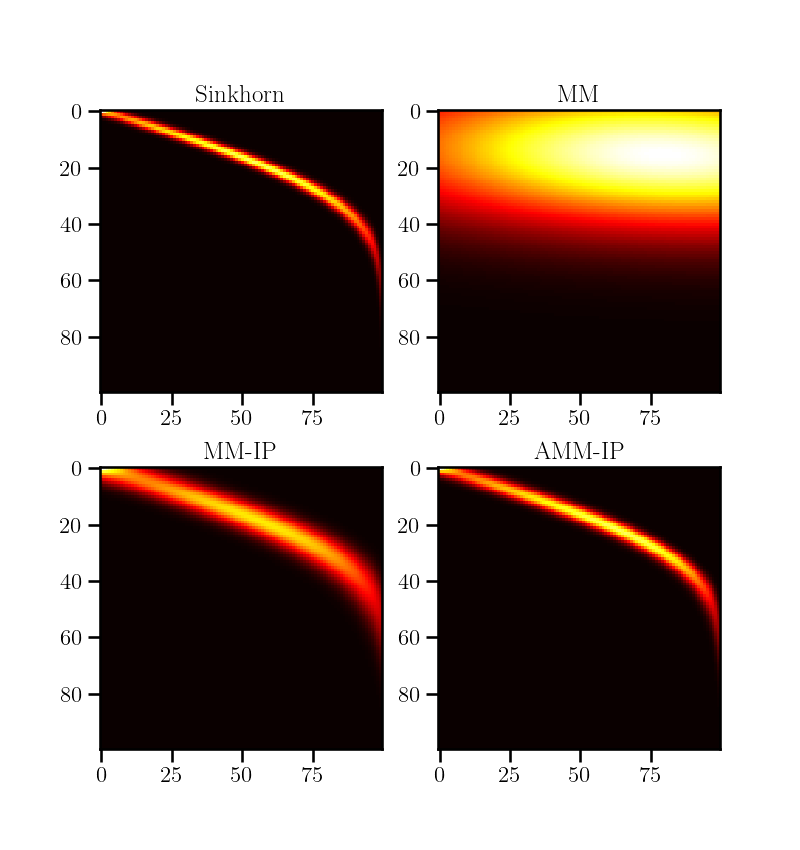
\includegraphics[width = 0.8\linewidth]{pic/ex2}
\setlength{\belowcaptionskip}{-10pt}
\caption{Comparing of the solutions obtained using different optimization methods, MM algorithm fails to accurately capture the sparse tendency of the solution in the UOT problems. MM-IP and AMM-IP methods perform significantly better, producing solutions similar to Sinkhorn's.}
\label{Fig:ex2}
\end{figure}

\section{Conclusion}
Overall, our experimental results illustrate the effectiveness of our proposed Inexact Penalized MM algorithm (MM-IP). Compared to the MM algorithm, our proposed method can effectively handle the challenge of larger $\tau$ values by utilizing an inexact penalization process that avoids poor initialization. This results in a superior solution quality that is competitive with the widely-known Sinkhorn algorithm. In the future, we plan to incorporate our expertise in the field of ALM to further accelerate the MM algorithm.

\bibliographystyle{jsai}
\bibliography{ref}

%%











